\section{Syntax}

\subsection{Text}

Display text in \textbf{bold}, \textit{italic}, \texttt{typewriter} \cite{overleaf_font}.

Embed website links with \href{https://www.overleaf.com/learn/latex/Hyperlinks}{displaying text}, \url{https://www.overleaf.com/learn/latex/Hyperlinks} \cite{overleaf_link}.

Use different formats of list to display \cite{overleaf_list}:
\begin{itemize}
    \item item 1
        \begin{enumerate}
            \item item 1
                \begin{description}
                    \item[Bold title] item 1
                \end{description}
        \end{enumerate}
\end{itemize}

Use special characters like \ding{52}, \ding{56} \cite{pifont}.

Embed code from file as figure, as shown in \Cref{fig:embed_ef,fig:embed_pf}.
\begin{figure}[H]
\lstinputlisting[
    language=Bash,
    showspaces=false,
    basicstyle=\ttfamily\footnotesize,
    numbers=left,
    numberstyle=\tiny,
    commentstyle=\color{gray},
]{../script/example.sh}
\caption{Embed entire script file.}
\label{fig:embed_ef}
\end{figure}
\begin{figure}[H]
\lstinputlisting[
    linerange={3-4},
    language=Bash,
    showspaces=false,
    basicstyle=\ttfamily\footnotesize,
    numbers=left,
    numberstyle=\tiny,
    commentstyle=\color{gray},
]{../script/example.sh}
\caption{Embed selected lines script file.}
\label{fig:embed_pf}
\end{figure}

\subsection{Figure}

Various tools can be use to create figures and are roughly classified as 1 (best) to 3 (worst) in \autoref{table:fig_tool}.

\begin{center}
    \captionof{table}{Assessment of different tools to create figures.}
    \label{table:fig_tool}
    \begin{tabular}{ c c c c c c }
        \toprule
        Tool & Time required & Ease of use & Adjustability & Image quality & Scripting \\
        \midrule
        Mermaid (PDF) \cite{mermaid} & 1 & 1 & 3 & 1 & 1 \\
        draw.io (PDF) \cite{drawio} & 2 & 1 & 2 & 1 & 3 \\
        GNU Plot (PDF) \cite{gnuplot} & 3 & 3 & 1 & 1 & 1 \\
        MS PowerPoint & 2 & 1 & 2 & 3 & 3 \\
        \LaTeX\ TikZ \cite{tikz} & 3 & 3 & 1 & 1 & 1 \\
        \bottomrule
    \end{tabular}
\end{center}

To embed a downloaded figure or figure created with external tools mentioned in \autoref{table:fig_tool}, the following format can be used for PNG, JPG and PDF (best quality) format \cite{inserting_img}.

\begin{figure}[H]
    \centering
    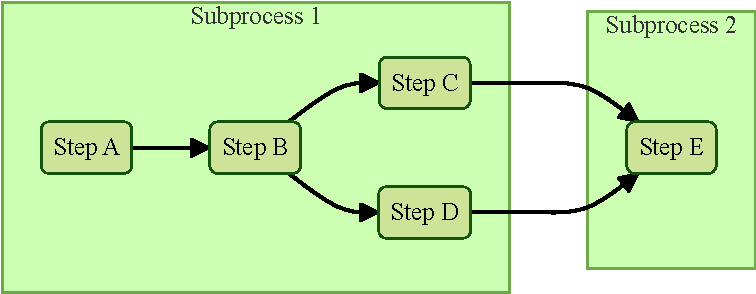
\includegraphics[width=0.8\textwidth]{../figure/mermaid_out/flowchart.pdf}
    \caption{A example of embedding a PDF image.}
    \label{fig:embed_pdf}
\end{figure}

To use TikZ in \LaTeX, visit the Minimal Working Example (MWE) example page \cite{tikz_example}. Additional packages will be needed and should be added in the \texttt{main.tex} file.

\subsection{Table}
% - table generator https://www.tablesgenerator.com/
% - combine rows
% - combine columns
\subsection{Equation}
\subsection{Algorithm}
\subsection{Citation}
% - bib file
% - get BibTeX information
% - BibTeX template
% - natbib
% - special case: some characters makes multiple page from pp. to present as p.
\subsection{Hyperlink}
% - citation, citeauthor
% - figure, table, section
% - multi-reference syntax
\subsection{Custom commands and additional packages}
% - renew reference name (Fig. Tab. Eq. Alg.)
% - keywords, keywordscn
% - add additional layer: paragraph
% - enquote
% - nth
% - xurl

\clearpage
